\chapter{General discussion, future work and conclusions}
\label{ch:conc}
\acresetall

%Discovery-driven or observation-driven vs hypothesis driven
%The full extent of diversity of the microbial world is still largely unexplored.
Antarctic lakes are exceptional ecosystems that contain microbial life adapted to extreme polar conditions and the local lake geochemistry.
Metagenomics has proven to be an effective way to map the diversity of lake ecosystems and provide hints of how they work.
In combination with metaproteomics and abiotic parameters, 
the work described in this thesis has made significant contributions to understanding ecosystem functions of Ace Lake and Organic Lake.
The most noteworthy achievement has been to describe taxa and microbial processes previously unknown to occur in these lakes, and from these descriptions, generate testable hypotheses of population and ecosystem level function.

\section{Summary of outcomes from this work}
%This has necessitated the development of new ways to extract biological inferences from complex datasets.
The overall objective of this thesis was to study Antarctic lake ecosystems using an integrative metagenomics driven approach.
In order to do this, methods were developed in chapter \ref{ch:ace} to measure properties of the community that would work alongside metagenomic sequencing to piece together a comprehensive description of ecosystem structure and function.
An epifluorescene microscopy protocol was designed that makes use of 0.01 \textmu{}m pore-size \ac{PCTE} membrane filters.
Using this protocol, cells and \acp{VLP} were successfully visualised and enumerated along the depth profile of Ace Lake, and subsequently in Organic Lake.
The need to develop this method was due to the discontinuation of supply of Anodisc filters, which are the standard filter used for direct counts of \acp{VLP} by epifluorescence microscopy.
Although cell and \ac{VLP} densities are fairly basic properties of the community, their measurement nonetheless revealed surprising results, such as the lack of correspondence between turbidity and cell density in Organic Lake.

A bioinformatic pipeline for analysis of metaproteomic mass spectra was also developed in chapter \ref{ch:ace} that incorporated use of matching metagenomic databases for protein identification and spectral counting to estimate protein abundances.
When applied to the metaproteomic analysis of Ace Lake, this workflow resulted in a greater number of protein identifications than previous work using the \ac{NR} and showed statistically significant functional differences between the strata of the lake.
It also described the functional capacity of dominant populations in the mixolimnion indicating specific adaptations to the Antarctic lake environment.
The elaboration of a conceptual framework incorporating genomic and functional data in the study Ace Lake laid the groundwork for the subsequent studies on Organic Lake.

In chapter \ref{ch:olv}, two near-complete \ac{OLPV} genomes and a complete \ac{OLV} genome were described.
Analysis of the \ac{OLV} genome indicated it was a new member of the virophage virus family that obligately utilise a  giant `helper' virus to complete their replication cycle, but which impair their helper's infectivity in the process.
Genomic comparison between \ac{OLV} and \ac{OLPV} identified shared regions that strongly suggest \ac{OLV} is a virophage of \ac{OLPV}.
The metaproteomic analysis identified both viral capsids confirming members of the population were actively replicating viruses and not, for example, accessory genetic elements.
The availibility of \textsc{DNA} sequences from the whole community meant the most likely host, \emph{Pyramimonas}, could be identified from the \ac{SSU} genes.
The inferred interaction of the \ac{OLV}, \ac{OLPV} and host was used to generate a model of their population dynamics that showed if \ac{OLV} acts as a `predator of a predator', this would lead to increased frequency of population cycling.
This was hypothesized to function in the Antarctic lake ecosystem as means to increase dissolved carbon release and secondary production over the summer season.
Potential relatives of the \ac{OLV} were also found in Ace Lake and in other aquatic environments indicating virophage may play an influential role in other ecosystems.

In chapter \ref{ch:org} a profile of the Organic Lake microbial taxonomic composition and potential for nutrient cycling was determined.
The community was found to consist primarily of eucaryotic algae related to \emph{Dunaliella} and three heterotrophic bacterial genera: \emph{Marinobacter}, \emph{Roseovarius} and \emph{Psychroflexus}.
The suboxic bottom zone of Organic Lake additionally contained lower abundance populations of \emph{Firmicutes}, \emph{Deltaproteobacteria} and \emph{Epsilonproteobacteria}.
Examination of genes involved in carbon cycling indicated a net loss of carbon could occur as potential for carbon fixation was lower than for respiration.
However, genes for photo- and lithoheterotrophic pathways linked to the dominant bacterial lineages were abundant; in particular \ac{AAnP} genes were much higher than in any other aquatic environment surveyed.
Use of these energy sources instead of organic carbon was hypothesized to be a specific adaptation of the heterotrophic bacterial population to conserve carbon within the system.
The capacity for nitrogen cycling also showed a shift away from fixation and a predominance of recycling of reduced nitrogen compounds.
This was similarly hypothesized to function as a mechanism to limit nitrogen loss.
A targeted search for genes involved in \ac{DMS} conversions found an abundance of \ac{DMSP} lyase genes indicating lysis of \ac{DMSP} is the likely source of the high \ac{DMS} levels that has been detected in Organic Lake.
\ac{DMSP} lyase genes were linked to the \emph{Gammaproteobacteria} and \emph{Alphaproteobacteria} populations indicating \ac{DMSP} is an important carbon and energy source.
Unlike marine environments, \ac{DMSP} lyase genes were more abundant than \ac{DMSP} demethylase genes. 
The only other metagenomes to show comparably high abundance of \ac{DMSP} lyase were other hypersaline environments suggesting the DMSP lysis pathway is favoured in high salinity systems. 
%We have used theory to guide our work.

\section{New perspectives and possibilities for future work}
The work described in this thesis is part of a program that is pioneering the use of shotgun metagenomics and metaproteomics in Antarctic lakes \cite{Ng2010, Lauro2011, Yau2011} and the Southern Ocean \cite{Wilkins2012b, Grzymski2012, Williams2012a, Williams2012b}.
They represent the largest datasets of this kind obtained for these environments.
%Apart from a \ac{SSU} diversity study of Organic Lake sediment  \cite{Bowman2000b}, chapters \ref{ch:olv} and \ref{ch:org} have been the only molecular-based investigations of Organic Lake.
Therefore, much of this work has been a discovery-driven effort to establish a picture of the biotic composition and function of these communities.
Further studies taking a similar approach are necessary to evaluate community composition and function overtime, especially during the winter.
Bioinformatic pipelines and theoretical models, such as the metaproteomics workflow described in chapter \ref{ch:ace} and modified Lotka-Volterra model from chapter \ref{ch:olv}, can be applied to these subsequent studies.
Hypotheses generated concerning specific populations and functions of the community generated from our existing models of the Antarctic lakes can also be tested.
Some of these questions can be addressed by `-omics' approaches, especially targeted metagenomic analyses.
But for other specific questions, emerging technologies look to be promising (such as viral tagging, single cell genomics, single virus genomes) complementary techniques metagenomic sequencing.

%Work that could be done now.
%The metaproteome of Organic Lake.
%The Organic lake resample?
%Determine the rest of the viral diversity of the organic lake samples.


\subsection{Dynamics over time}
To establish a complete understanding of the Antarctic Lakes requires comprehensive descriptions of the microbial community over different time scales.
Obtaining metagenomic and functional metatranscriptomic or metaproteomic data from the lakes over the span of a year will provide an understanding of how the microbial community copes with the dramatic seasonal temperature, light and ice-cover changes.

In particular, it can elucidate how the community sustains itself in the winter when the absence of light is expected to forestall phototrophic primary production.
%Furthermore, it can determine what stategies phototrophic organisms employ to survive during this period.
Paired metagenomic and metaproteomic analyses of the coastal Southern Ocean detected dramatic changes between summer and winter \cite{Grzymski2012, Williams2012a}.
Winter samples were dominated by active chemolithoautotrophs including sulphur-oxidising \emph{Gammaproteobacteria} and ammonia oxidising \emph{Crenarcheaota} \cite{Grzymski2012, Williams2012b}.
If the lake ecosystem reflects that of the coastal Southern Ocean, chemolithoautrophs can be expected to similarly become dominant in the winter. 
Chemolithoautotrophs in the Organic Lake summer community included a small population of sulphur-oxidising \emph{Proteobacteria} that may become dominant in the winter.
No signatures for \emph{Crenarchaeota} or ammonia oxidation were present in Organic Lake.
Furthermore, if the model proposed for Organic Lake of short-circuiting the nitrogen cycle by avoiding oxidised nitrogen forms holds true, we can expect ammonia oxidising microorganisms will not play a part in the Organic community in the winter unless nitrogen fixing organisms similarly increase.
Whether the short burst of photosynthesis or sustained chemolithoautotrophy is the main source of primary production in the lakes can be ascertained by measuring rates of production over the season.

\subsubsection{Short time scales}
Strain cycling of the cyanobacteria?
Strain cycling of the OLV and OLPV?

\subsubsection{Interannual cycle}
What happens to the associated viral populations over the winter?
Interannual comparisons also need to be established to see how robust the community is over the long term.
Cite the long term studies showing steady reproducible annual time series.



%Sampling over a finer time-scale can establish the dynamics of target populations such as the \ac{OLV} and \ac{OLPV}. 

%Future experiments can look at fluorescence of bchlA
%\subsection{Enumeration of cells and \acp{VLP} }
%New methods have emerged in the enumeration of cells


\subsection{Virophages}
Since the discovery of the \ac{OLV} described in chapter \ref{ch:olv}, two other members of the virophage family have been reported.
The first of these is the Mavirus (for Maverick virus) so named for its evolutionary relationship with the Maverick/Politon class of eucaryotic transposons \cite{Fischer2011}.
Like Sputnik, Mavirus has an absolute requirement for coinfection with a helper virus, in this case \ac{CroV}, in order to replicate.
Also like Sputnik, addition of Mavirus during \ac{CroV} infection leads severe drops in production of \ac{CroV} \cite{Fischer2011}.
The other virophage reported was called Sputnik 2 (its genome is virtually identical to Sputnik) and like Sputnik was also found in association with strain of mimivirus, named lentille virus \cite{Desnues2012}.
But unlike Sputnik, Sputnik 2 was found both as a separate genome and integrated in the lentille virus genome \cite{Desnues2012}.
The availability of these new virophages in culture affords a new perspective on \ac{OLV} and virophages in general.

%\subsubsection{How many more virophages are out there?}
%We can try and reconstruct more virophage genomes from Ace Lake?

\subsubsection{Is \ac{OLV} really a `virophage'?}
The inability for Mavirus to infect without \ac{CroV} and its detrimental effect on \ac{CroV} just like Sputnik strengthens the assumption that OLV would similarly have a `virophage' phenotype \ac{OLPV}.
This is in part because Mavirus and \ac{CroV} and quite divergent from Sputnik and mimivirus respectively, yet retain the same traits \cite{Fischer2010, Fischer2011}, suggesting the `virophage' phenotype is common to the whole lineage.
Secondly, these cultured virophages offers some mechanistic reasons for why \ac{OLV} would function as the other virophages.
As both mimivirus and \ac{CroV} encode a great deal of their own replication and transcription machinery, including all \textsc{DNA} and \textsc{RNA} polymerase subunits, they do not localise to the nucleus during infection but generate the viral factory in the cytoplasm \cite{LaScola2008, Fischer2011}.
Sputnik and Mavirus replicate exclusively in the giant virus factory and make use of the helper virus replication and transcription systems \cite{LaScola2008, Fischer2011}.
Furthermore, Sputnik and Mavirus share the promoter and other transcriptional control sequences of their helper viruses \cite{Claverie2009, Fischer2011}.
They therefore are primarily parasitising the resources of the helper viruses, which seems a likely cause of reduced helper virus production \cite{Claverie2009, Fischer2011}.
\ac{OLPV}-1 encodes all eight \textsc{RNA} polymerase subunits (see GenBank accession HQ704802) indicating it, like all other members of the mimivirus lineage, would replicate solely in the cytoplasm.
Therefore, it is likely \ac{OLV} would exclusively utilise its helper virus' molecular machinery to similarly detrimental effect.
Ultimately, definitely determining if this is the case for the \ac{OLV} would require isolating it from the environment.

\subsubsection{What is the mode of infection of \ac{OLV}?}
Comparison of three different virophage genomes has raised tantalising questions about virophage physiology, evolution and ecology
%All three genomes have share homologues of the Sputnik V20 \ac{MCP}, V3 FstK-HerA DNA packaging ATPase and V9 putative cysteine protease but otherwise are quite divergent.
%Sputnik and Mavirus additionally share a the V13 primase/superfamily 3 helicase and the V14 Zn-ribbon domain containing protein.
%While Sputnik and \ac{OLV} share the V18/19 minor virion protein, V1 primase-polymerase containing protein and V21 hypothetical protein.
Mavirus, in particular, is in many ways more similar to the Maverick/Politon transposable elements in the possession of a retroviral-family integrase that is absent in Sputnik and \ac{OLV} \cite{Fischer2011}.
This was theorised to have been separately acquired as a way to stabilise the relationship between the ancestral Mavirus and its cellular host as integration of a virophage could perhaps serve as a defence against infection of the giant helper virus \cite{Fischer2011}.
In support of this, Mavirus can be independently phagocytosed by \emph{Cafeteria roenbergensis} in the absence of \ac{CroV} -- potentially to reduce the severity of a subsequent \ac{CroV} infection \cite{Fischer2011}.
As yet, Mavirus has not been reported to be integrated in the host \emph{Cafeteria roenbergensis}.
In contrast, Sputnik seems to associate directly with the fibrils that coat the mimivirus virion, not the host \emph{Acanthamoeba} cell \cite{Boyer2011}.

These two modes of infection, that is a virophage--host interaction followed by helper \emph{vs}. helper--virophage co-infection of host cell, would lead to distinct effects on the population dynamics in the environment.
Detection of \ac{OLV} genome as a separate circular molecular in the 0.8--0.1 \textmu{}m size fraction indicates it was captured in association with larger particles.
Determination of the mode of infection for \ac{OLV} would improve predictive modelling of \ac{OLV} driven impacts on algal blooms.
This could be achieved by observation of \ac{OLV}-\ac{OLPV} infections in culture if it can be isolated.
Another possibility is flow cytometric sorting of sample populations of potential hosts and \ac{OLPV} from the environment and screening of the presence of \ac{OLV}.
The latter experiment would also establish fundmental properties of \ac{OLV} such as the identity of hosts and helper viruses, proportions of infected cells and proportions of \ac{OLPV} infections that include an \ac{OLV}.

\subsubsection{Can \ac{OLV} integrate into its helper?} 
The discovery that Sputnik 2 can integrate into its helper lentille virus suggests a similar interaction could occur between \ac{OLV} and \ac{OLPV}.
This is because integration of Sputnik 2 is localised to a 352 bp region corresponding to the Sputnik V6 gene that encodes a collagen-like repeat-containing protein that is shared by Sputnik 2, lentille virus and mamavirus  \cite{Desnues2012} 
\ac{OLV} and \ac{OLPV} shared a homologous collagen-like repeat-containing protein (Chapter\ref{ch:olv}) that may similarly function as a site of integration.
As yet, the conditions and mechanism by which Sputnik 2 integrates is unknown.
From the metagenomic sequence, \ac{OLV} assembled as a separate molecule (Chapter\ref{ch:olv}).
Screening of metagenomic assemblies from other sampling dates, such as Ace lake and the 2008 Organic Lake samples, for \ac{PV} genomes with integrated virophages can be performed to see if this occurs in the environment at different times.
Again, obtaining isolates or assembling more \ac{PV} genomes can determine if this is a common trait in other virophage systems.
If integration occurs between \ac{OLV} and \ac{OLPV} it would have interesting implications for their natural dynamics.
One interesting possibility is that integration of virophages may function analogously to lysogeny in bacteriophages if integration lead to a `dormant' state for the virophage.
In this scenario, virophages would then integrate into their helper virus when helper virus densities are low to avoid driving their helpers to extinction.
On the other hand, if integration does not entail dormancy of the virophage, it could function as a means to ensure transmission.

%%%OLV distribution and evolution questions
%virophages seem to attack only mimivirus relatives.
%How common are they in the environment?
%They seem like an ancient lineage, how widespread are they? Do they infect other NCLDV


\subsection{Functional analyses in the Organic lake community}
%Need to show that AAnP genes are expressed with RT-PCR, proteomics

%Cloning of the dddD, dddL genes into appropriate host to show activity.
%Look for inputs into the lake.
%Is allochtonous inputs feeding the lake?
%Need to show the dynamics of the lake
%Need to look at the rest of viral community 



\section{Perspectives on `-omics' approaches }
It was not so long ago that what could be called the second molecular revolution in microbial ecology began in earnest with they first shotgun metagenomic sequences of a marine virome \cite{Breitbart2002}.
That metagenome, sequenced with Sanger sequencing technology, was a modest 1.28 Mbp \cite{Breitbart2002}.
The first shotgun sequenced metagenomes of cellular life from the Sargasso Sea \cite{Venter2004} and the Iron Mountain acid mine drainage \cite{Tyson2004} added 265 Mbp and 76 Mbp respectively to the public databanks.

Since the availability of next generation high-throughput sequencing technologies, the volume of data has increased exponentially and is continuing to rise.
A single sample from the Antarctic lake datasets described in this thesis sequenced by the Roche GS-FLX titanium sequencer is 140 Mbp, while a recent study using Applied Biosystems SOLiD sequencing of a marine sample \cite{Iverson2012} analysed 55,000 Mbp -- close to 400 times the amount of data.
This illustrates just how quickly sequencing technology advancing that each new study essentially has to develop new ways of looking into the microbial milieu captured in their particular dataset.
The benefits of using high-throughput sequencing technologies means that shotgun metagenomics will continue to be used as tool in the foreseeable future.
But it also means encountering tough analytical challenges that comes with it.

With higher throughput and falling costs of sequencing, genomic projects are finding analytical bottle necks are occuring in computational analysis.
This is because availability of computational resources and scaling-up of algorithms to multiple genomes or computing clusters is not occurring as quickly as the amount of sequencing.
Metagenomic sequencing projects entail a minimum level of processing that includes data clean-up, assembly, \ac{ORF} prediction, clustering and generally \ac{BLAST} like comparisons before biological interpretations can be made.
The most intensive of these is the sequence comparisons to known databanks.
With the sheer volume of next generation sequencing datasets, this type of analysis requires a supercomputer to process.
Local cluster computing has thus far been a standard way to process metagenomic datasets. 
Acquiring the necessary computational resources can work out more costly for groups expecting only the sporadic use.
The volumes of data can also overwhelm the capabilities of single computation clusters \cite{Iverson2012}.
This has been addressed to some extent by use of webserver pipelines specialised in metagenomic processing such as \ac{MG-RAST} \cite{Meyer2008} and \ac{CAMERA} \cite{Sun2011} for cellular metagenomes as well as \textsc{Metavir} \cite{Roux2011} and \textsc{VIROME} \cite{Wommack2012} for viral metagenomes. sea star?
These webserver pipelines take on the burden of maintaining the programs, hosting the databases and the computational requirements of the users.
However, these workflows are generally not customisble if the user's needs fall too far outside of that provided. 
For example, requiring different comparative databases, alternative programs or handling sequence data types.
Further, processing massive datasets may still take unfeasibly long time.
cloud computing resources \cite{}
to do this is a realistic time frame can be extremely challenging.

% Limitations of bioinformatic tools themselves.Gene prediction needs to get better. de novo assembly, binning.
%De novo assembly need to improve to be able to tackle highly diverse populations.
% eg. Iverson.
% Having high sequencing depth, a simple target population
% Could a metagenome ever be really `closed' metagenome, unless it is the most simple community, it seems difficult to imagine.

%Biological limitations, interpreting of the biology is only as good at the data bases. requires good recording of metadata.
%A lucky tail, discovery of the virophage was only possible with the presence of the Sputnik in 2008. If databases from 2007 were used, it simply would have been an abundant unknown molecule, likely not even recognisably viral.
%Similarly, if dddD and dddL genes were not in the databases at the right time, they would not be seen.
%In some ways metagenomic data still contains an 'unseen majority. Particularly viral metagenomes.
%' the difference is that all this information can be a resource that is reanalysed.

 
%%Metaproteomics
%Highly dependent on having a matching metagenome
%Compared to metagenomics, relatively data poor as a lot of the spectra cannot be matched
%But spectra can be reanalysed

%%Future of -omics studies will have to go beyond just sequencing and sequencing more.
% Need to have studies over long time scales, and finer spatial resolutions.
% Need to marry with emerging technologies that are able to target specific individuals or populations at high resolution
% Spatial resolution has begun with microfluidics systems (Seymour), 
% digital PCR to associate, single cell genomics, targetted metagenomics with viral tagging, SIP
% It also requires a lot of old fashioned microbiology like isolation fed back in from microbiology to have model systems in the lab.
% Ultimately, these technologies are tools that we are just learning to use
%\figref{fig:prok_diversity} illustrates how much additional bacterial and archaeal taxonomic diversity has been revealed by environmental sequencing and also suggests how much more of their genomic diversity is still undescribed. 
%\begin{figure}[H]
\centering
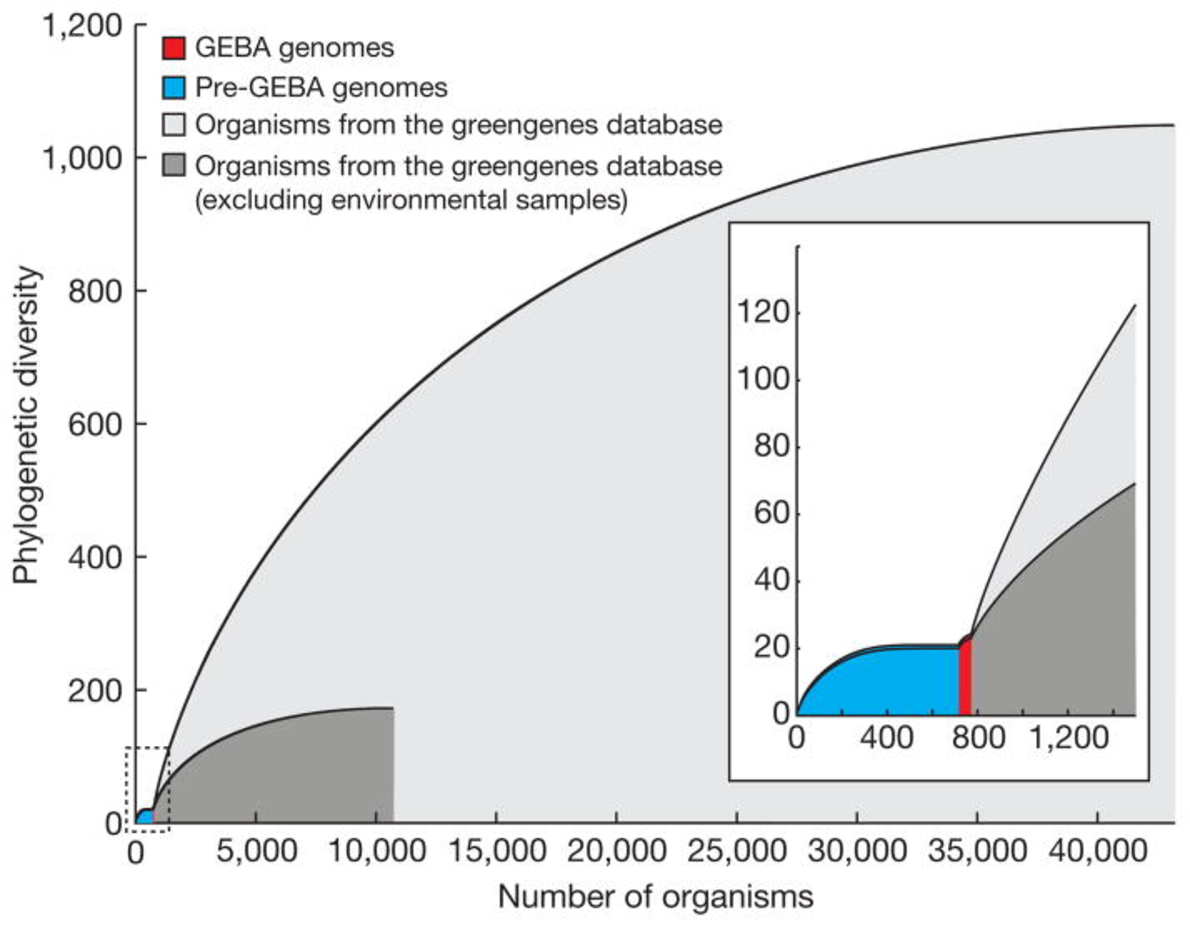
\includegraphics[width=100mm]{conc_figures/prok_diversity.pdf}
\caption[Plot of the diversity of \emph{Bacteria} and \emph{Archaea} from \citet{Wu2009}]{ Plot of the diversity of \emph{Bacteria} and \emph{Archaea} from \citet{Wu2009}. 
The diversity as shown by sequencing of 16S \acp{SSU} genes from the environment, from known organisms and from genomes is compared.
The inset shows the diversity encompassed from sequenced genomes before and after the Genomic Encyclopedia of \emph{Bacteria} and \emph{Archaea} (GEBA) sequencing project, which targets genomes for sequencing based on phylogenetic diverisity \cite{Wu2009}.
}
\label{fig:prok_diversity}

\end{figure}


\section{Concluding remarks}
%Molecular data can be continued to be mined! 
%Serves as a record for prosterity
%Metagenomics is not enough! There needs to be functional data, single cell data, biochemical data.

